\section{تحلیل آماری و تصویرسازی داده‌های زمان اجرای الگوریتم‌ها}
در این بخش، هدف بررسی هوشمند و پویای داده‌های مربوط به زمان اجرای سه الگوریتم مختلف بر حسب اندازه داده‌های ورودی از محدوده $ 100 $ الی $ 600 $ کیلوبایت و تحلیل تغییرات رفتار آن‌ها پس از افزودن سطر جدید $ 700 $ کیلوبایت است. تمامی این مراحل بدون هاردکد کردن داده‌ها و از طریق توابع پانداس\footnote{\lr{Pandas}} انجام شده است.

\subsection{مراحل و نحوه پیاده‌سازی الگوریتم‌ها}
مراحل پیاده‌سازی این بخش در زبان پایتون\footnote{\lr{Python}} به شرح زیر است:
\begin{enumerate}
    \item \textbf{فراخوانی پویا:} با استفاده از تابع \lstinline|pd.read_excel|، فایل داده‌ها مستقیماً خوانده شده و با متد \lstinline|str.strip| نام ستون‌ها پاک‌سازی می‌شوند تا فواصل خالی احتمالی باعث ایجاد خطا در محاسبات نگردند.
    \item \textbf{محاسبه شاخص‌های آماری:} پیش از اعمال تغییرات در ساختار فایل، میانگین ستون مربوط به الگوریتم ۲ محاسبه و ثبت می‌شود.
    \item \textbf{تزریق پویای داده‌ی جدید:} ردیف جدید مربوط به داده‌ی $ 700 $ کیلوبایت به کمک تابع \lstinline|pd.concat| به انتهای ماتریس داده‌ها افزوده می‌شود تا در اجرای مجدد، نمودارها به صورت خودکار به‌روزرسانی شوند.
    \item \textbf{تولید نمودارها:} با بهره‌گیری از کتابخانه‌های مت‌پلات‌لیب\footnote{\lr{Matplotlib}} و سی‌بورن\footnote{\lr{Seaborn}}، سه نمودار خطی، میله‌ای و جعبه‌ای برای تحلیل همه‌جانبه توزیع و روند داده‌ها رسم می‌شوند.
\end{enumerate}

\subsection{کد پایتون پیاده‌سازی شده}
کد کامل پایتون توسعه‌یافته برای این بخش به صورت زیر است:

\begin{latin}
\begin{lstlisting}
import pandas as pd
import matplotlib.pyplot as plt
import seaborn as sns

# Set style for professional-looking plots
sns.set_theme(style="whitegrid")

# 1. Reading the Excel file dynamically
excel_file = 'پروژه 3.xlsx'
df = pd.read_excel(excel_file)
df.columns = df.columns.str.strip()

# 2. Calculating the mean for Alg.2 (Before adding the new data row)
mean_alg2 = df['Alg.2'].mean()
print("--- Part 2 (c): Statistical Analysis ---")
print(f"Mean execution time for Alg.2 (100KB to 600KB): {mean_alg2:.2f}\n")

# 3. Dynamically appending new data row (700KB row)
new_row = {
    'Run time for different data size': '700KB',
    'Alg.1': 80,
    'Alg.2': 320,
    'Alg.3': 700
}
df = pd.concat([df, pd.DataFrame([new_row])], ignore_index=True)
print("--- Part 2 (b): Updated Dataframe with 700KB Row ---")
print(df)
print("\n")

size_col = df.columns[0]
algorithms = [col for col in df.columns if col != size_col]

# 4. Plotting Bar, Line, and Box Plots
# Line Plot
plt.figure(figsize=(10, 6))
for alg in algorithms:
    plt.plot(df[size_col], df[alg], marker='o', linewidth=2, label=alg)
plt.title('Execution Time Trend across Different Data Sizes', fontsize=14, fontweight='bold')
plt.xlabel('Data Size', fontsize=12)
plt.ylabel('Execution Time (ms)', fontsize=12)
plt.legend()
plt.tight_layout()
plt.savefig('execution_time_line_plot.png', dpi=300)

# Bar Plot
df_long = pd.melt(df, id_vars=[size_col], value_vars=algorithms, var_name='Algorithm', value_name='Execution Time')
plt.figure(figsize=(10, 6))
sns.barplot(data=df_long, x=size_col, y='Execution Time', hue='Algorithm', palette='muted')
plt.title('Comparison of Algorithm Execution Times per Data Size', fontsize=14, fontweight='bold')
plt.xlabel('Data Size', fontsize=12)
plt.ylabel('Execution Time (ms)', fontsize=12)
plt.tight_layout()
plt.savefig('execution_time_bar_plot.png', dpi=300)

# Box Plot
plt.figure(figsize=(8, 6))
sns.boxplot(data=df[algorithms], palette='pastel')
plt.title('Distribution of Execution Times per Algorithm', fontsize=14, fontweight='bold')
plt.xlabel('Algorithm', fontsize=12)
plt.ylabel('Execution Time Range', fontsize=12)
plt.tight_layout()
plt.savefig('execution_time_box_plot.png', dpi=300)
\end{lstlisting}
\end{latin}

\subsection{خروجی دقیق برنامه در محیط ترمینال}
متن خروجی حاصل از محاسبات و چاپ ماتریس داده‌ها به شرح زیر است:

\begin{latin}
\begin{verbatim}
--- Part 2 (c): Statistical Analysis ---
Mean execution time for Alg.2 (100KB to 600KB): 250.00

--- Part 2 (b): Updated Dataframe with 700KB Row ---
  Run time for different data size  Alg.1  Alg.2  Alg.3
0                            100KB     50    200    100
1                            200KB     55    220    200
2                            300KB     60    240    300
3                            400KB     65    260    400
4                            500KB     70    280    500
5                            600KB     75    300    600
6                            700KB     80    320    700
\end{verbatim}
\end{latin}

\subsection{تحلیل آماری میانگین زمان اجرا}
مطابق با خواسته بند «ج» پروژه، میانگین زمان اجرای مربوط به الگوریتم ۲ برای اندازه‌های اولیه داده‌ها ($ 100 $ تا $ 600 $ کیلوبایت) بر اساس فرمول زیر محاسبه شده است:
\[
\mu = \frac{1}{N}\sum_{i=1}^{N} X_i = \frac{200 + 220 + 240 + 260 + 280 + 300}{6} = 250.00\,\text{ms}.
\]
این شاخص آماری نشان می‌دهد که رفتار کلی الگوریتم ۲ در بازه داده‌های ورودی استاندارد، حول مرکز ثقل $ 250 $ میلی‌ثانیه نوسان می‌کند.

\subsection{نمودارهای ترسیم شده و تحلیل جامع رفتار الگوریتم‌ها}
نمودارهای زیر خروجی‌های تصویری به‌دست‌آمده از کد پایتون هستند که پس از تزریق خودکار داده‌ی سطر $ 700 $ کیلوبایت ترسیم شده‌اند.

\begin{figure}[htbp]
    \centering
    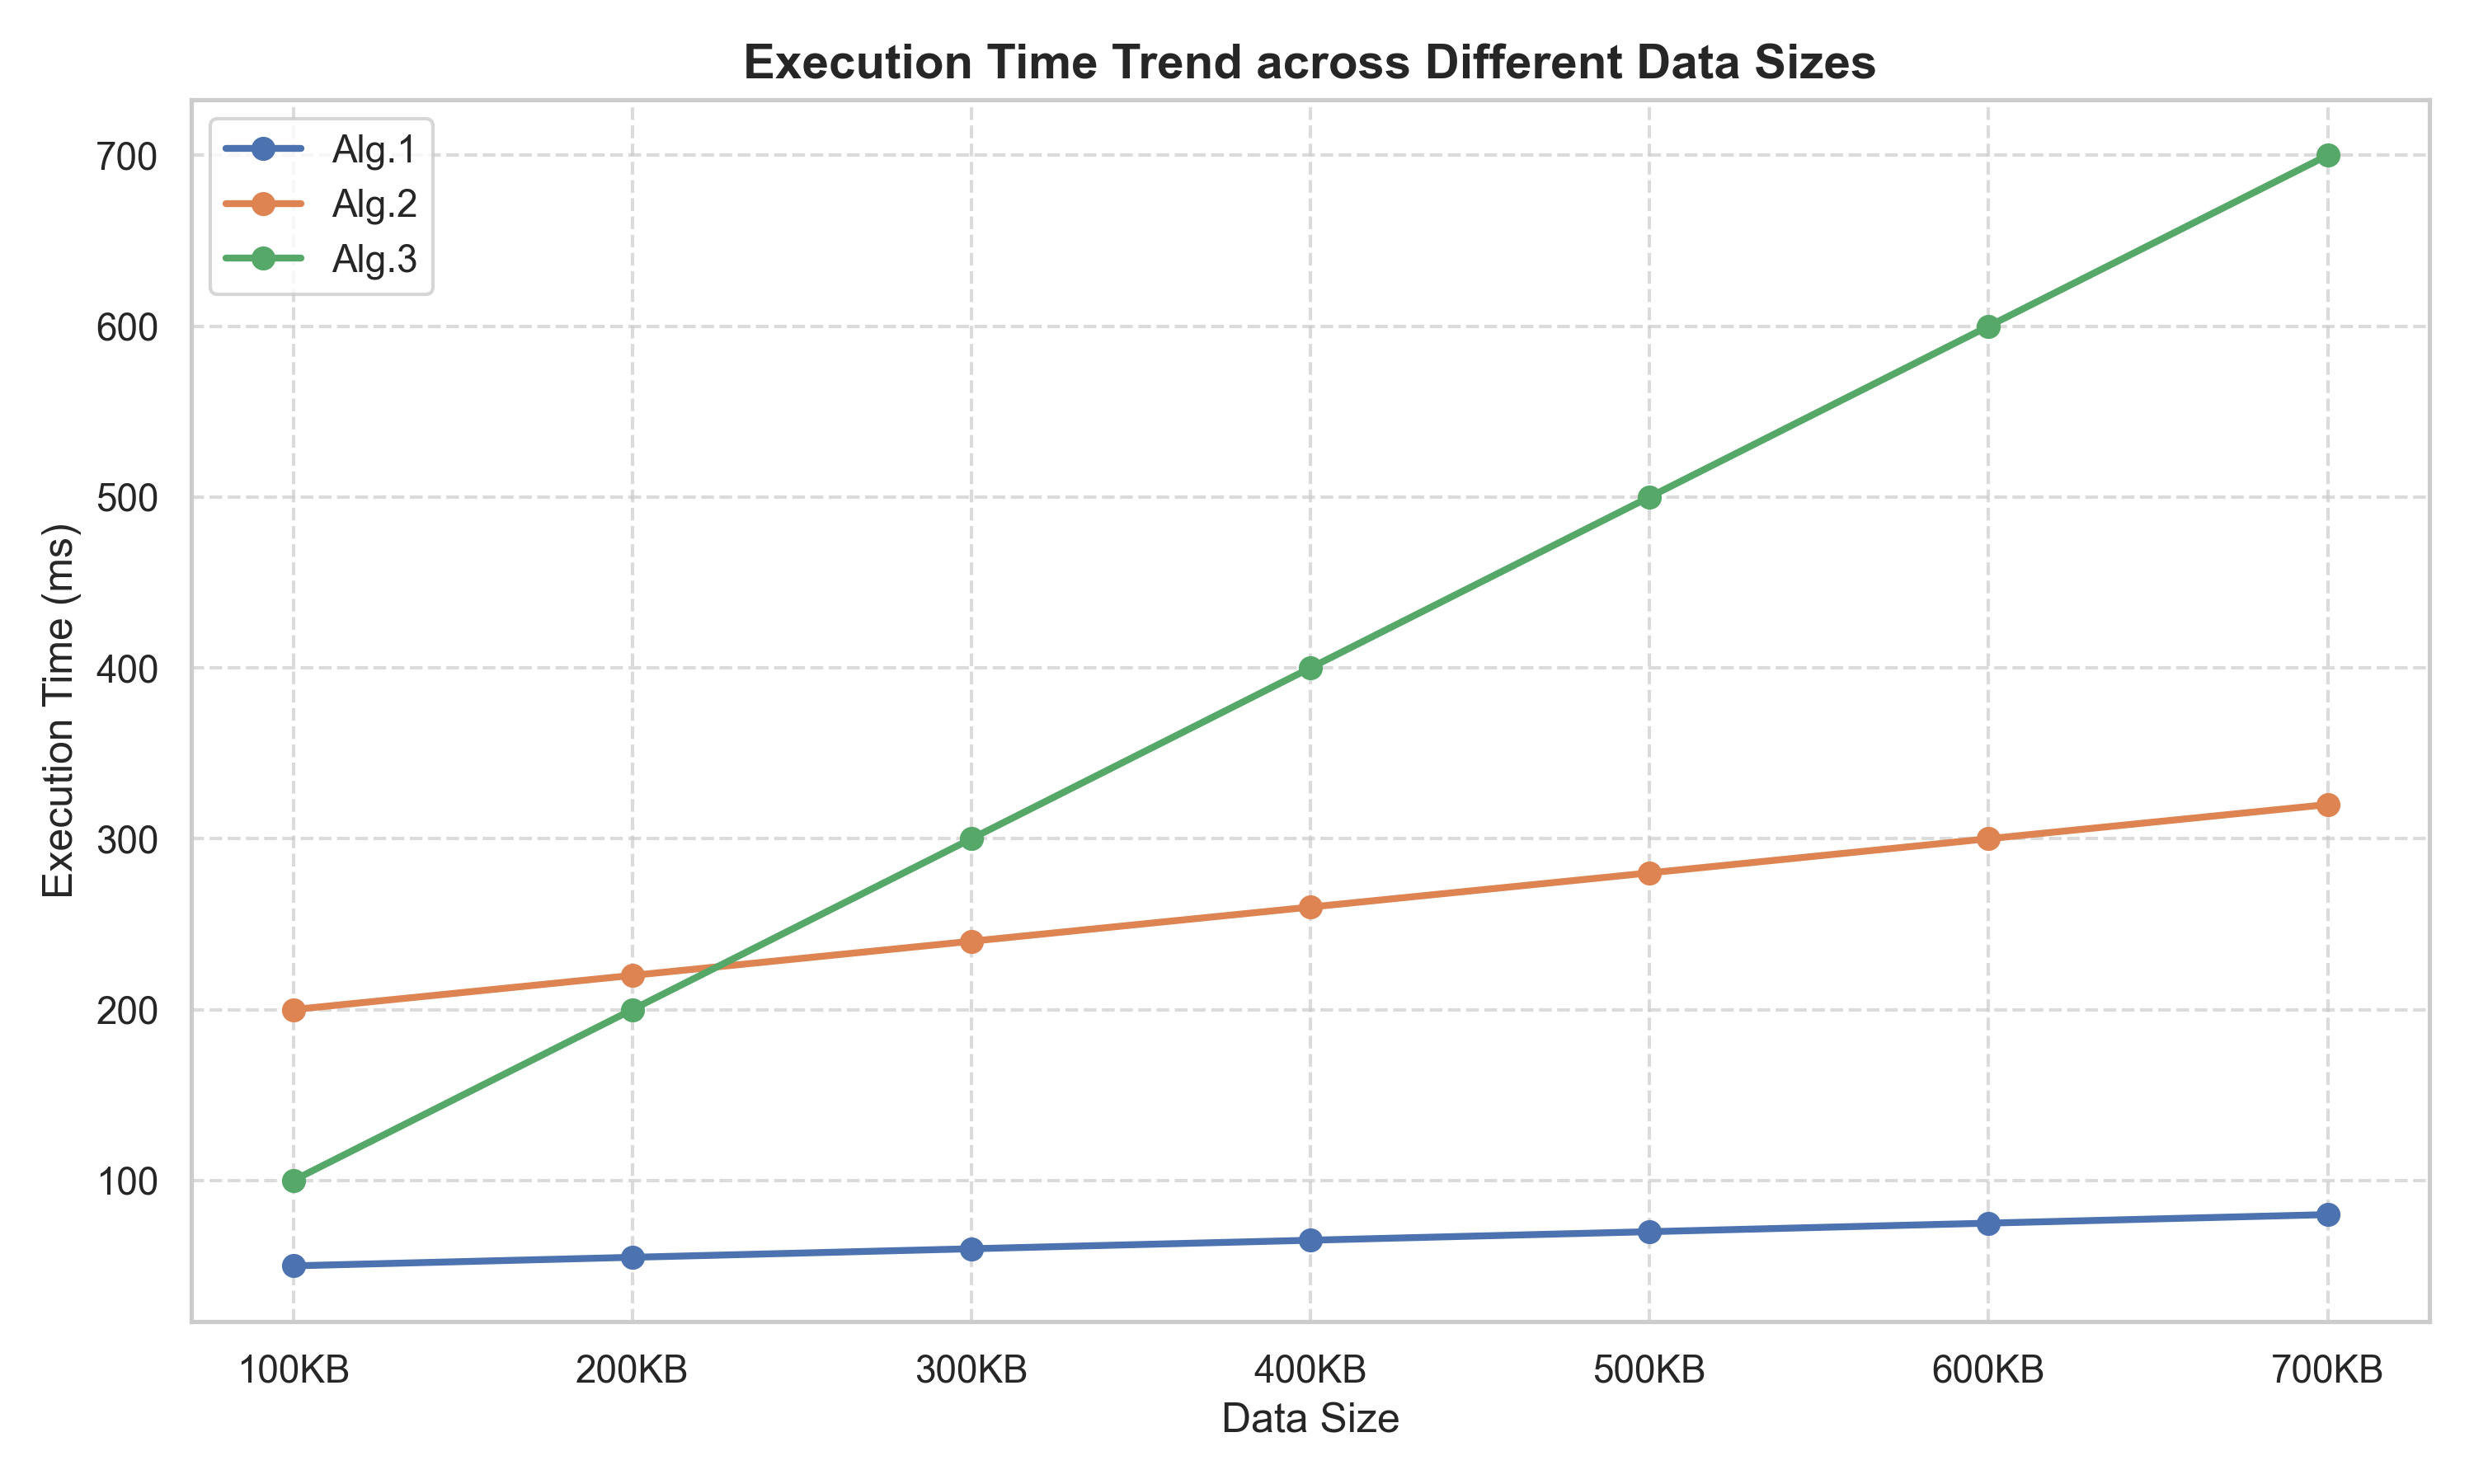
\includegraphics[width=0.85\textwidth]{execution_time_line_plot.png}
    \caption{روند تغییرات زمان اجرای الگوریتم‌ها بر حسب افزایش اندازه ورودی.}
    \label{fig:line_plot}
\end{figure}

\begin{figure}[htbp]
    \centering
    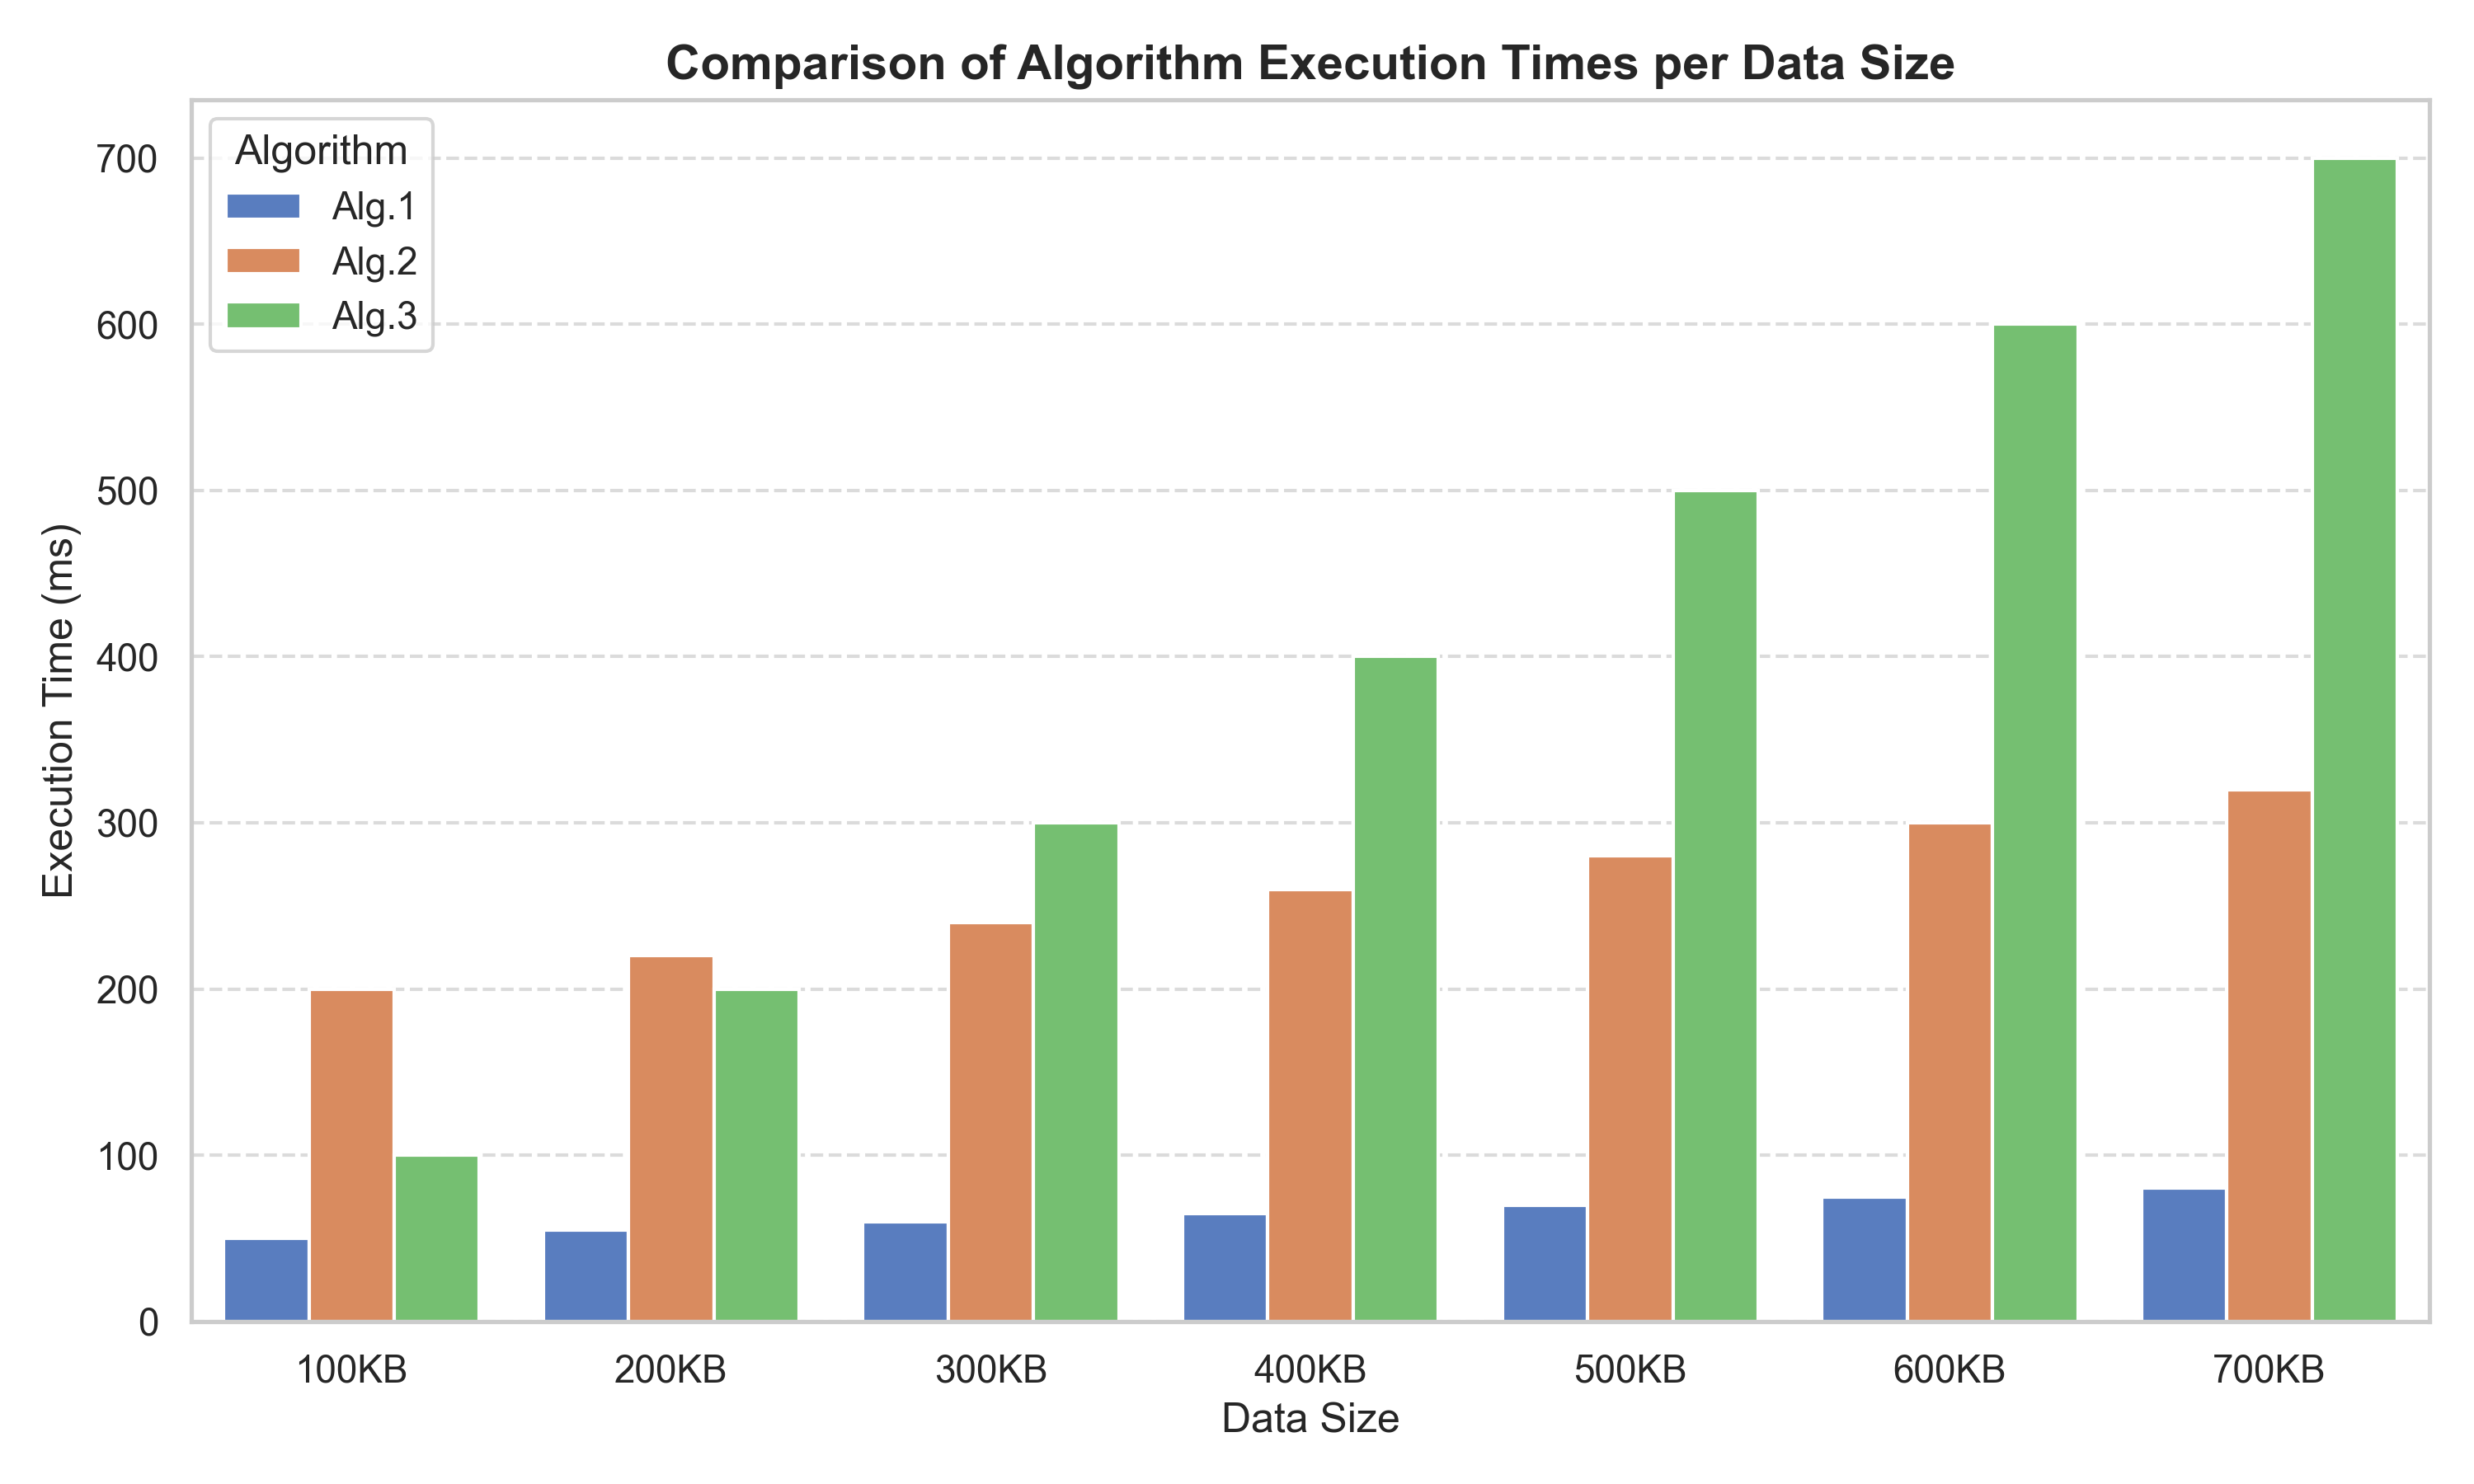
\includegraphics[width=0.85\textwidth]{execution_time_bar_plot.png}
    \caption{مقایسه ستونی و چندگانه زمان اجرای الگوریتم‌ها در هر یک از سطوح اندازه داده.}
    \label{fig:bar_plot}
\end{figure}

\begin{figure}[htbp]
    \centering
    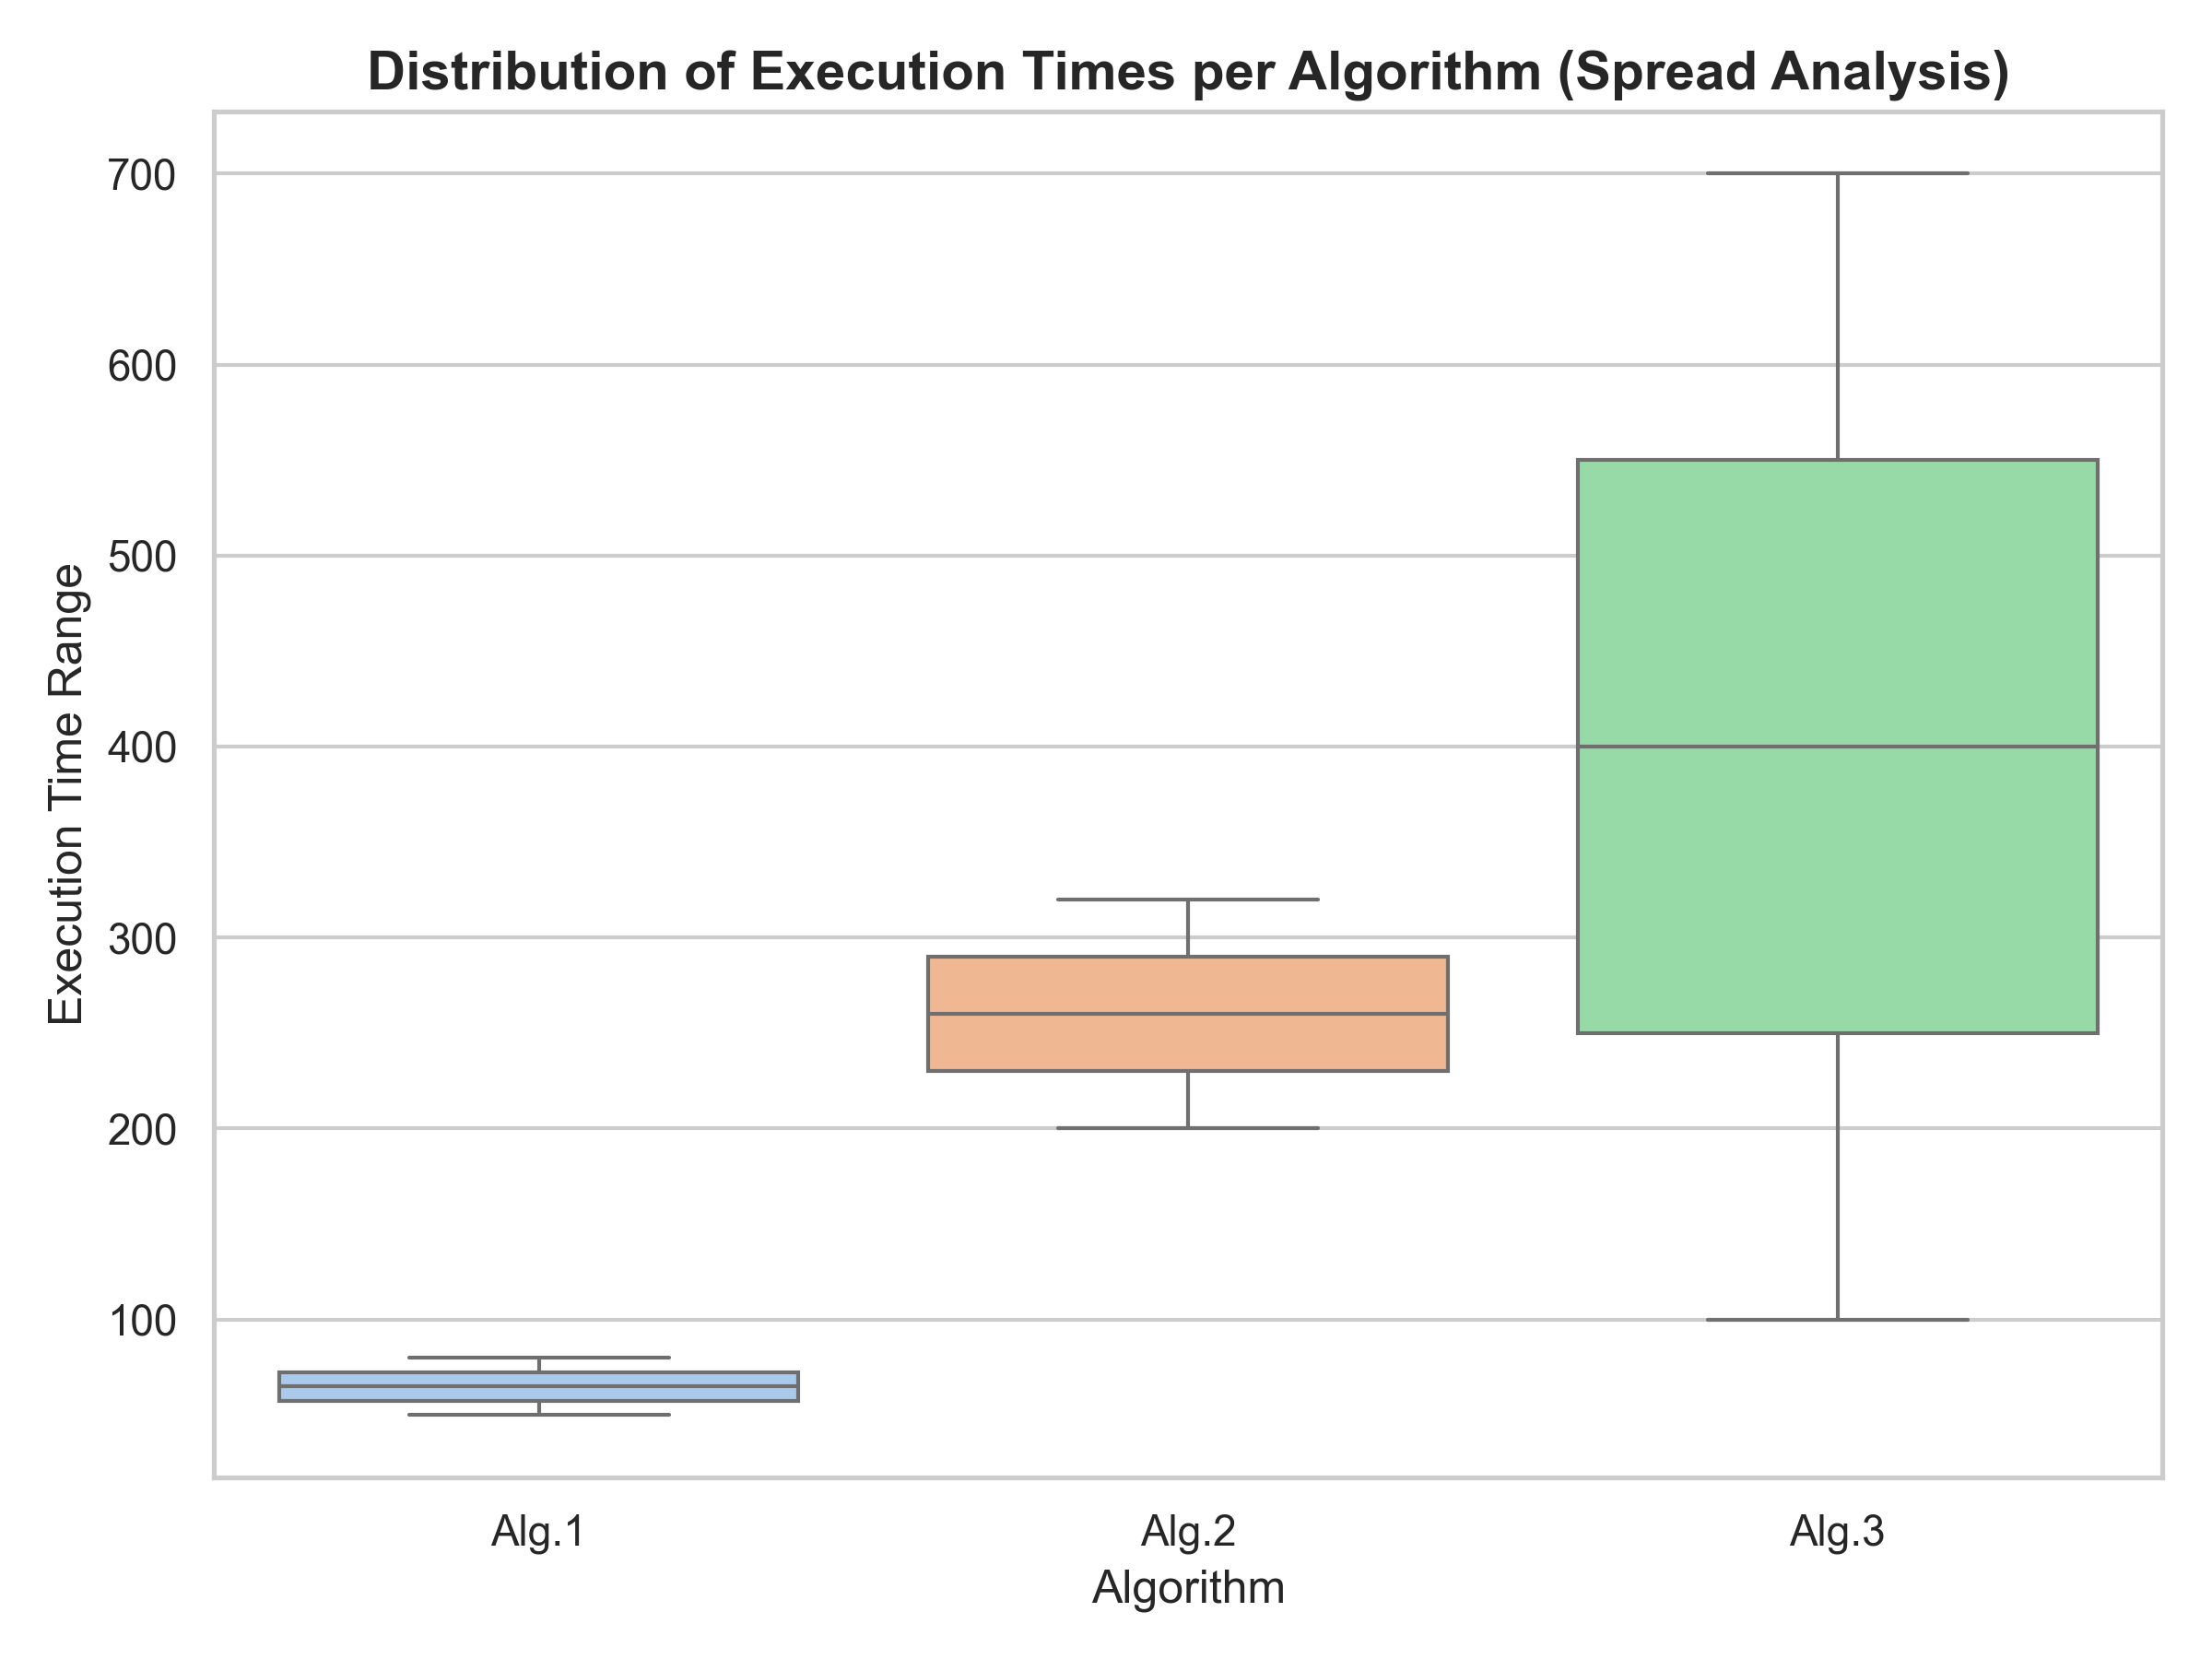
\includegraphics[width=0.7\textwidth]{execution_time_box_plot.png}
    \caption{نمودار جعبه‌ای تحلیل دامنه توزیع، میانه و پراکندگی کلی زمان اجرای الگوریتم‌ها.}
    \label{fig:box_plot}
\end{figure}

\subsubsection{تحلیل نمودار خطی و بررسی روند رشد}
با توجه به شکل~\ref{fig:line_plot}، رفتار رشد زمان اجرای هر سه الگوریتم به وضوح قابل تحلیل است:
\begin{itemize}
    \item \textbf{الگوریتم ۱:} این الگوریتم با شیبی بسیار ملایم رشد می‌کند و در تمام طول آزمایش کمترین زمان اجرا را به خود اختصاص داده است؛ در نتیجه، بهینه‌ترین الگوریتم از نظر پیچیدگی زمانی\footnote{\lr{Time Complexity}} است.
    \item \textbf{الگوریتم ۲:} روندی کاملاً خطی و با شیب ثابت دارد. اگرچه زمان شروع آن از الگوریتم ۳ در حجم‌های کوچک بیشتر است، اما نرخ رشد کنترل‌شده‌ای دارد.
    \item \textbf{الگوریتم ۳:} این الگوریتم دارای تندترین شیب صعودی است. زمان اجرای آن با افزایش اندازه ورودی به شدت بالا می‌رود و حالت ناپایداری در حجم‌های بزرگ پیدا می‌کند.
\end{itemize}

\subsubsection{تحلیل نمودار میله‌ای و مقایسه نقطه‌ای عملکرد}
بر اساس شکل~\ref{fig:bar_plot}، در اندازه‌های ورودی کوچک مانند $ 100 $ و $ 200 $ کیلوبایت، الگوریتم ۳ سریع‌تر از الگوریتم ۲ عمل می‌کند. اما یک نقطه تلاقی مهم در محدوده $ 300 $ کیلوبایت رخ می‌دهد. از حجم $ 400 $ کیلوبایت به بعد، الگوریتم ۲ گوی سبقت را از الگوریتم ۳ می‌رباید؛ چرا که زمان اجرای الگوریتم ۳ به شکل تصاعدی افزایش یافته و در حجم $ 700 $ کیلوبایت به اوج خود یعنی $ 700 $ میلی‌ثانیه می‌رسد. این امر عدم مقایس‌پذیری\footnote{\lr{Scalability}} الگوریتم ۳ را اثبات می‌کند.

\subsubsection{تحلیل نمودار جعبه‌ای و بررسی ثبات توزیع}
نمودار جعبه‌ای در شکل~\ref{fig:box_plot}، دامنه تغییرات داده‌ها را به تصویر می‌کشد:
\begin{itemize}
    \item جعبه مربوط به الگوریتم ۱\footnote{\lr{Alg.1}} بسیار فشرده و در پایین‌ترین سطح قرار دارد که نشان‌دهنده پایداری بالا، انحراف معیار ناچیز و واریانس بسیار کم در شرایط کاری مختلف است.
    \item جعبه مربوط به الگوریتم ۳\footnote{\lr{Alg.3}} بیشترین ارتفاع (طول بازه مابین چارک اول و سوم) را دارد. این گستردگی نشان‌دهنده حساسیت فوق‌العاده بالا و عدم ثبات زمان اجرای این الگوریتم نسبت به تغییر ابعاد ورودی سیستم است.
\end{itemize}
